% \documentclass[13pt]{beamer}
\documentclass[handout,13pt]{beamer}

\usepackage{pgfpages}  % Uncomment one of these lines for X-on-1 printing
% \pgfpagesuselayout{4 on 1}[letterpaper, border shrink=5mm, landscape]
% \pgfpagesuselayout{2 on 1}[letterpaper, border shrink=5mm]

\usepackage{ifthen}
\newboolean{show_handout_comments}  % Uncomment one of the below
% \setboolean{show_handout_comments}{true}  % Show handout-only comments
\setboolean{show_handout_comments}{false}  % Hide comments

\usepackage{graphicx}
\usepackage{color}
\usepackage{enumerate}
\usepackage{bm}
\usepackage{listings}

\usepackage{booktabs}
\usepackage{multirow}

\usepackage{amsmath}
\usepackage{amssymb}
\usepackage{amsthm}
\usepackage{mathtools}
\usepackage{dsfont}
\usepackage{subfigure}
\usepackage{tikz}
\usetikzlibrary{bayesnet}


\usetheme{Madrid}
\usecolortheme{beaver}

\setbeamertemplate{enumerate items}[circle]  % standard enumeration
\setbeamertemplate{itemize items}[circle]  % default itemize
\setbeamertemplate{navigation symbols}{}

% Resuming lists across frames
\newcounter{savedenum}
\newcommand*{\saveenum}{\setcounter{savedenum}{\theenumi}}
\newcommand*{\resume}{\setcounter{enumi}{\thesavedenum}}

% Comments
\newcommand*{\comment}[2][red]{%
  \ifthenelse{\boolean{show_handout_comments}}{
  \only<beamer:0>{\textcolor{#1}{\footnotesize #2}}}{}}

% Boxes
\makeatletter
\newcommand*{\colbox}[2][black]{\textcolor{#1}{%
  \fbox{\normalcolor\m@th$\displaystyle#2$}}}
\makeatother

\newcommand*{\combox}[3][black]{%
  \mbox{\begin{tabular}[t]{@{}c@{}}
    $\colbox[#1]{\displaystyle#2}$\\
    \textcolor{#1}{\scriptsize #3}
    \end{tabular}}}

\newcommand*{\coltextbox}[2][black]{\textcolor{#1}{%
  \setlength{\fboxrule}{1pt}\fbox{\normalcolor#2}}}

\newcommand*{\answerbox}[2][black]{%
  \only<1|handout:0>{#2} \only<2>{\coltextbox[#1]{#2}}}

%%%%%%%%%%%%%%%%%%%%%%%%%%%%%%%%%%%%%%%%%%%%%%%%%%%%%%%%%%%%%%%%%%%%%%%%%%%%%%
% User-defined LaTeX commands
\DeclareMathOperator*{\Cov}{Cov}
\DeclareMathOperator*{\Var}{Var}
\DeclareMathOperator*{\argmax}{arg\,max}
\DeclareMathOperator*{\argmin}{arg\,min}
\DeclarePairedDelimiter{\abs}{\lvert}{\rvert}
\DeclarePairedDelimiter{\norm}{\lVert}{\rVert}
\newcommand*{\ttilde}{{\raise.17ex\hbox{$\scriptstyle\sim$}}}
\newcommand*{\foralls}{\ \forall \ }
\newcommand*{\E}{\mathbb E}
\newcommand*{\R}{\mathbb R}
\newcommand*{\I}{\mathds{1}}
\newcommand*{\Prob}{\mathbb P}
\newcommand*{\notorth}{\ensuremath{\perp\!\!\!\!\!\!\diagup\!\!\!\!\!\!\perp}}
\newcommand*{\orth}{\ensuremath{\perp\!\!\!\perp}}
\newcommand*{\dif}{\,\mathrm{d}}
\newcommand*{\Dif}[1]{\,\mathrm{d^#1}}
\newcommand*{\e}{\mathrm{e}}
\newcommand*{\m}[1]{\textbf{#1}}
\newcommand{\cond}{\;\ifnum\currentgrouptype=16 \middle\fi|\;}
\newcommand*{\bmath}[1]{\boldsymbol{#1}}
\newcommand*{\yestag}{\addtocounter{equation}{1}\tag{\theequation}}
\newcommand*{\notaligned}[1]{\noalign{$\displaystyle #1$}}

\makeatletter
\newsavebox{\mybox}\newsavebox{\mysim}
\newcommand*{\distas}[1]{%
  \savebox{\mybox}{\hbox{\kern3pt$\scriptstyle#1$\kern3pt}}%
  \savebox{\mysim}{\hbox{$\sim$}}%
  \mathbin{\overset{#1}{\kern\z@\resizebox{\wd\mybox}{\ht\mysim}{$\sim$}}}%
}
\makeatother
\newcommand*{\dist}{\sim}
\newcommand*{\distiid}{\distas{\text{i.i.d}}}

\newcommand*{\convas}[1]{\xrightarrow{#1}}
\newcommand*{\conv}{\convas{}}

\makeatletter
\def\moverlay{\mathpalette\mov@rlay}
\def\mov@rlay#1#2{\leavevmode\vtop{%
  \baselineskip\z@skip \lineskiplimit-\maxdimen
  \ialign{\hfil$\m@th#1##$\hfil\cr#2\crcr}}}
\newcommand{\charfusion}[3][\mathord]{
  #1{\ifx#1\mathop\vphantom{#2}\fi\mathpalette\mov@rlay{#2\cr#3}}
  \ifx#1\mathop\expandafter\displaylimits\fi}
\makeatother
\newcommand{\cupdot}{\charfusion[\mathbin]{\cup}{\cdot}}
\newcommand{\bigcupdot}{\charfusion[\mathop]{\bigcup}{\cdot}}
%%%%%%%%%%%%%%%%%%%%%%%%%%%%%%%%%%%%%%%%%%%%%%%%%%%%%%%%%%%%%%%%%%%%%%%%%%%%%%


\title[601 Final Project]{Hillary Clinton Emails}
\author[Leland Bybee, Roger Fan, Ryan Vaughn]{Leland Bybee, Roger Fan, Ryan Vaughn}
% \institute[]{}
\date{\today}


\begin{document}


\begin{frame}
\maketitle
\end{frame}


\begin{frame}{Data}
\begin{itemize}
\item From 2008 to 2013, Hillary Clinton and some of her staff used a private email server for much of their communication
\item In response to FOIA requests, the State Department has released pdfs of roughly 30,000 of these emails, with roughly 8,000 sent by Clinton
\item We mostly want to condense and explore the data
  \begin{itemize}
  \item Break down a huge interpretation problem to a human-sized one
  \item Find specific and relatable observations, not just statistical ones
  \end{itemize}
\end{itemize}
\end{frame}


\begin{frame}{Data}
\begin{itemize}
\item We have a dataset of all these released emails, including sender and receiver information\footnote{Thanks to Ben Hamner and the WSJ for making their code and data available, respectively.}
\pause\item Bag-of-words model
  \begin{itemize}
  \item Stemming: combining words with the same ``root''
  \item Remove extremely rare words and extremely common (stop) words
  \end{itemize}
\item After cleaning, roughly 28,000 emails and a total vocabulary of over 3,000 words
\end{itemize}
\end{frame}


\begin{frame}{Visualization}
\begin{itemize}
\item In order to visualize these emails, we first need a measure of distance
\item Cosine similarity:
  \begin{equation*}
  \cos(\phi) = \frac{<V, W>}{\norm{V}\norm{W}}
  \end{equation*}
\item We can then use classical multi-dimensional scaling to visualize this data in lower dimensions
\end{itemize}
\end{frame}


\begin{frame}{Visualization}
\begin{figure}[h]
\centering
\subfigure[2D]{\label{fig:mds_2d}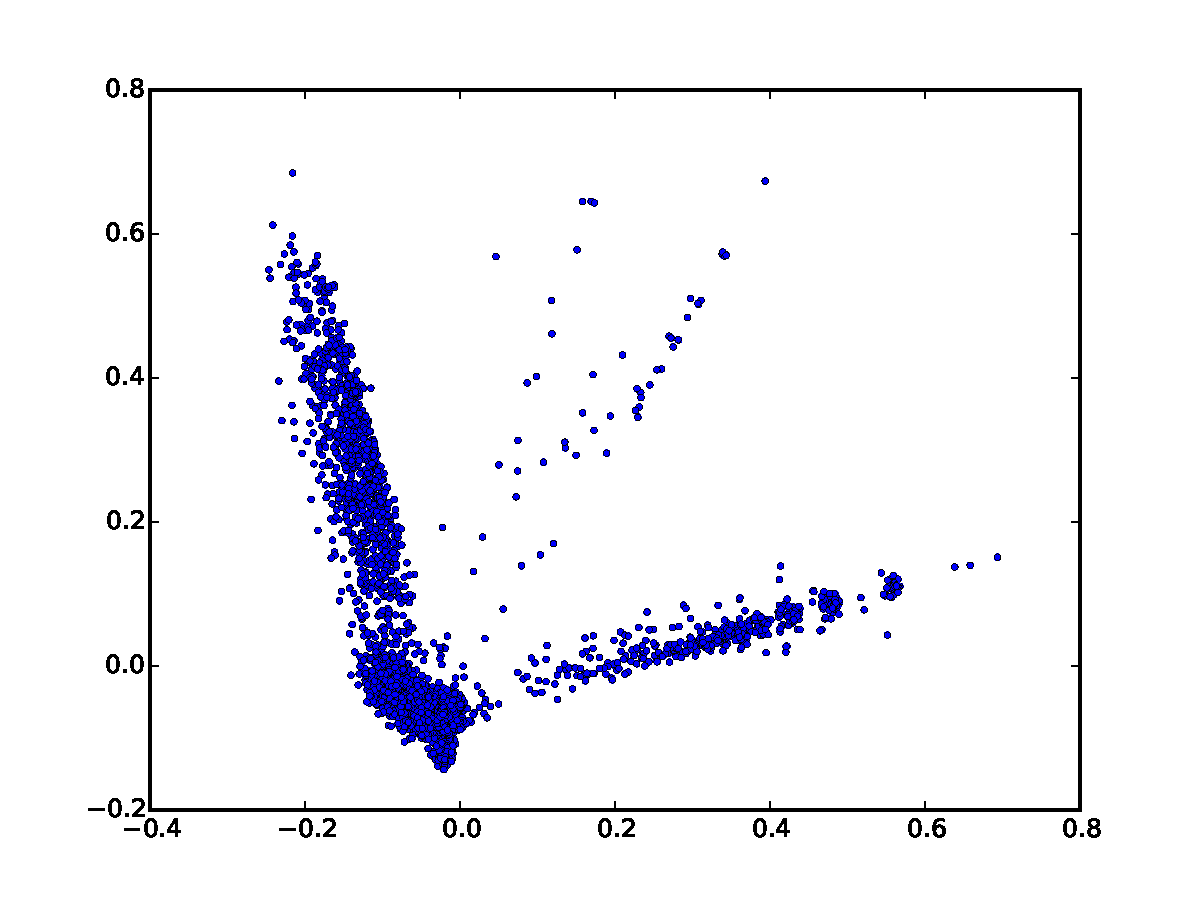
\includegraphics[width=0.44\linewidth]{../images/mds_2d.pdf}}
\subfigure[3D]{\label{fig:mds_3d}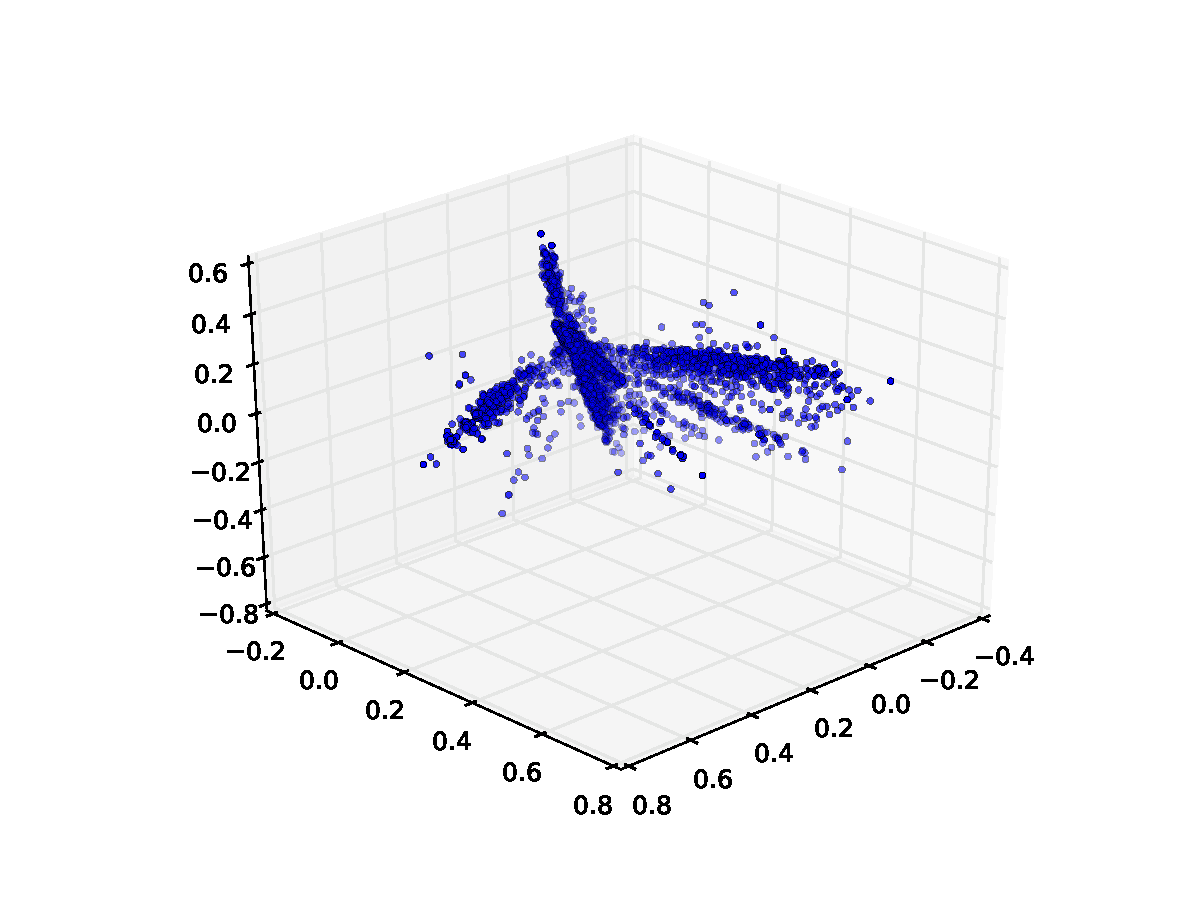
\includegraphics[width=0.54\linewidth]{../images/mds_3d_1.pdf}}
\label{fig:mds}
\end{figure}
\end{frame}


\begin{frame}{Spectral Clustering}
\begin{itemize}
\item Cluster points using their pairwise similarity
\item Computer the first $K$ eigenvectors of the normalized Laplacian
  \begin{equation*}
  L = I - D^{-1/2} S D^{-1/2}
  \end{equation*}
\item Perform $k$-means clustering on the resulting eigenvectors
\end{itemize}
\end{frame}


\begin{frame}{Spectral Clustering}
\begin{figure}[h]
\centering
\subfigure[2D]{\label{fig:cluster_2d}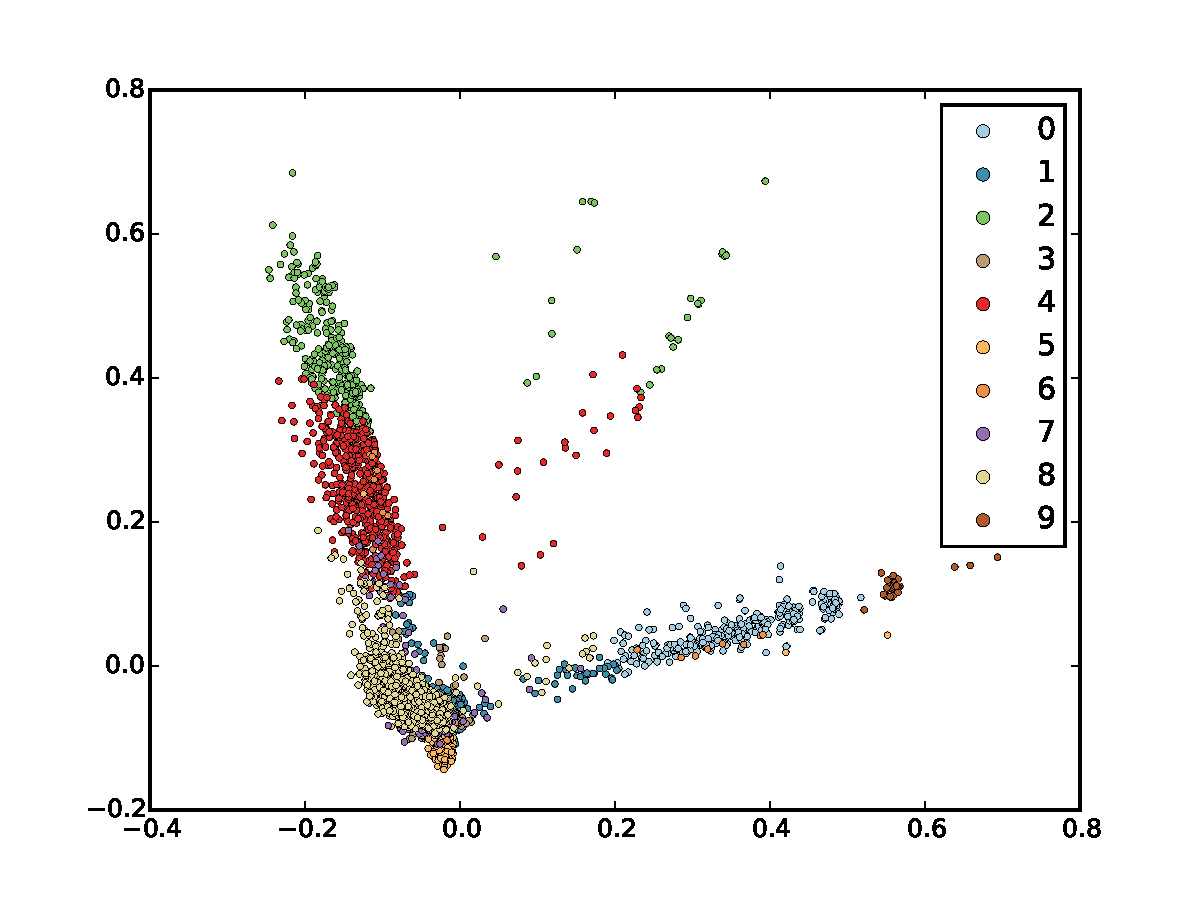
\includegraphics[width=0.44\linewidth]{../images/mds_2d_cluster.pdf}}
\subfigure[3D]{\label{fig:cluster_3d}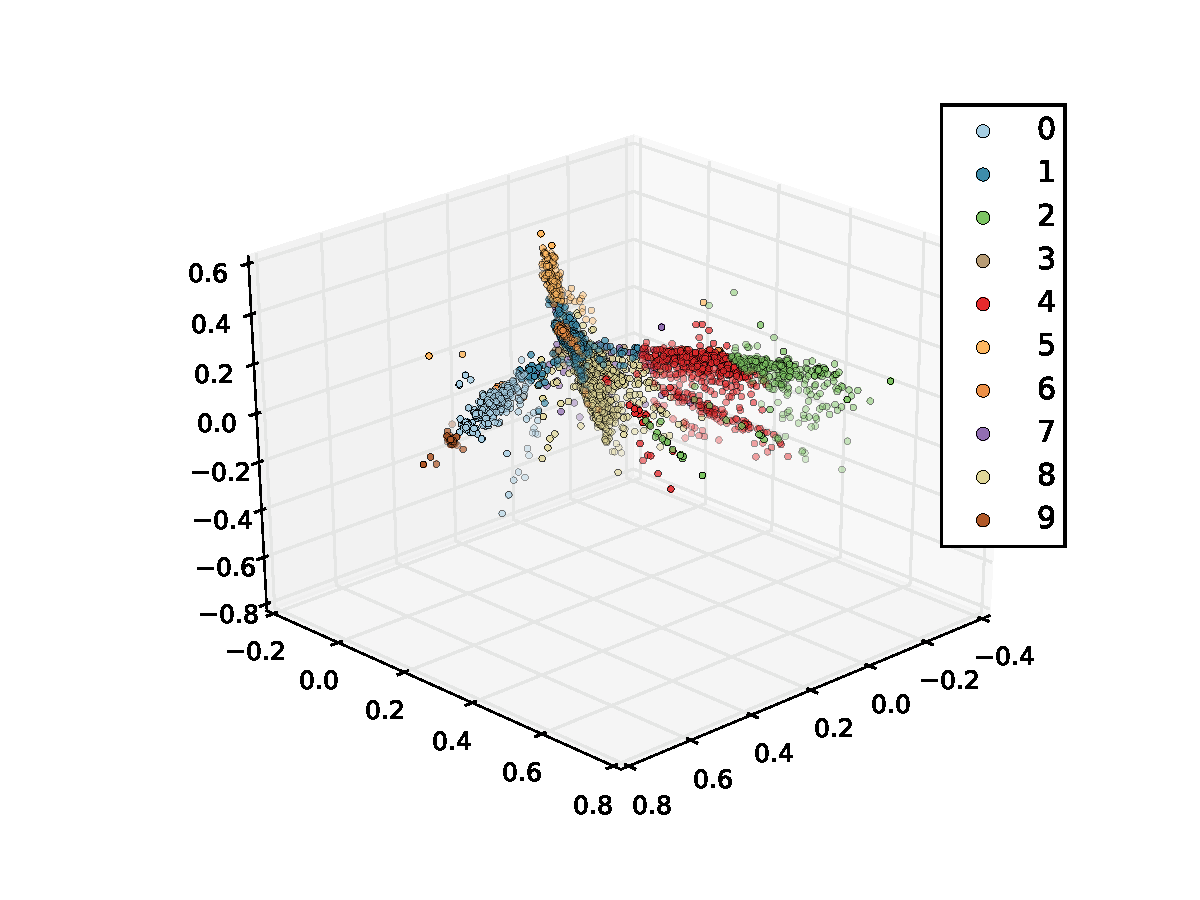
\includegraphics[width=0.54\linewidth]{../images/mds_3d_cluster_1.pdf}}
\label{fig:cluster}
\end{figure}
\end{frame}


\begin{frame}{Latent Dirichlet Allocation}
\begin{figure}
\centering
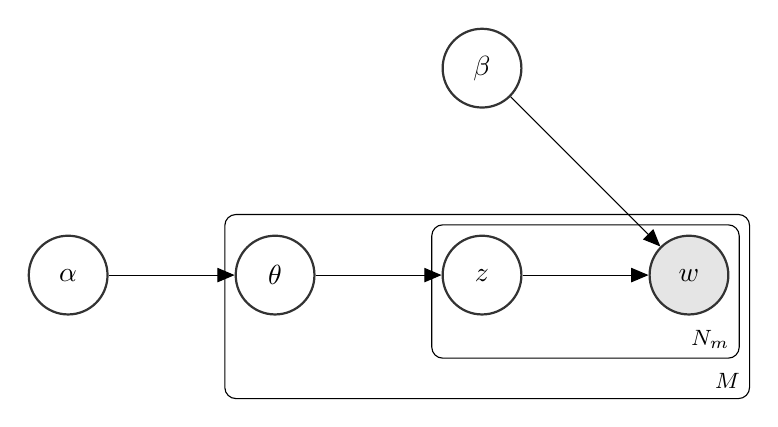
\begin{tikzpicture}[scale=1.0, every node/.style={transform shape}]
\tikzstyle{main}=[circle, minimum size = 10mm, thick, draw =black!80, node distance = 16mm]
\tikzstyle{connect}=[-latex, thick]
\tikzstyle{box}=[rectangle, draw=black!100]
  \node[main] (alpha) {$\alpha$};
  \node[main] (theta) [right=of alpha] {$\theta$};
  \node[main] (z) [right=of theta] {$z$};
  \node[main] (beta) [above=of z] {$\beta$};
  \node[main, fill=black!10] (w) [right=of z] {$w$};
  \edge {alpha} {theta};
  \edge {theta} {z};
  \edge {z,beta} {w};
  \plate {words} {(z)(w)} {$N_m$};
  \plate {docs} {(theta)(z)(w)(words.south east)(words.north west)} {$M$};
\end{tikzpicture}
\end{figure}
\end{frame}


\begin{frame}{Latent Dirichlet Allocation: Some Details}
\begin{itemize}
\item We use $K = 30$ topics for our resulting model.
\item What we ultimately care about are $\theta$ and $\beta$.
\item $\theta$ corresponds to how likely a topic is to appear in a document.
\item $\beta$ corresponds to how likely each word is to be associated with each topic.
\end{itemize}
\end{frame}


\begin{frame}{Latent Dirichlet Allocation: Some Details}
\begin{itemize}
\item Some questions we want to answer with LDA
\begin{itemize}
\item Can we see sensible topics in the LDA output?
\item What are the most common topics of the emails?
\item Do the topics for each email line up with real world events?
\item Can we associate email senders with topics?
\end{itemize}
\end{itemize}
\end{frame}


\begin{frame}{Exploring Topics}
\begin{figure}[h]
\centering
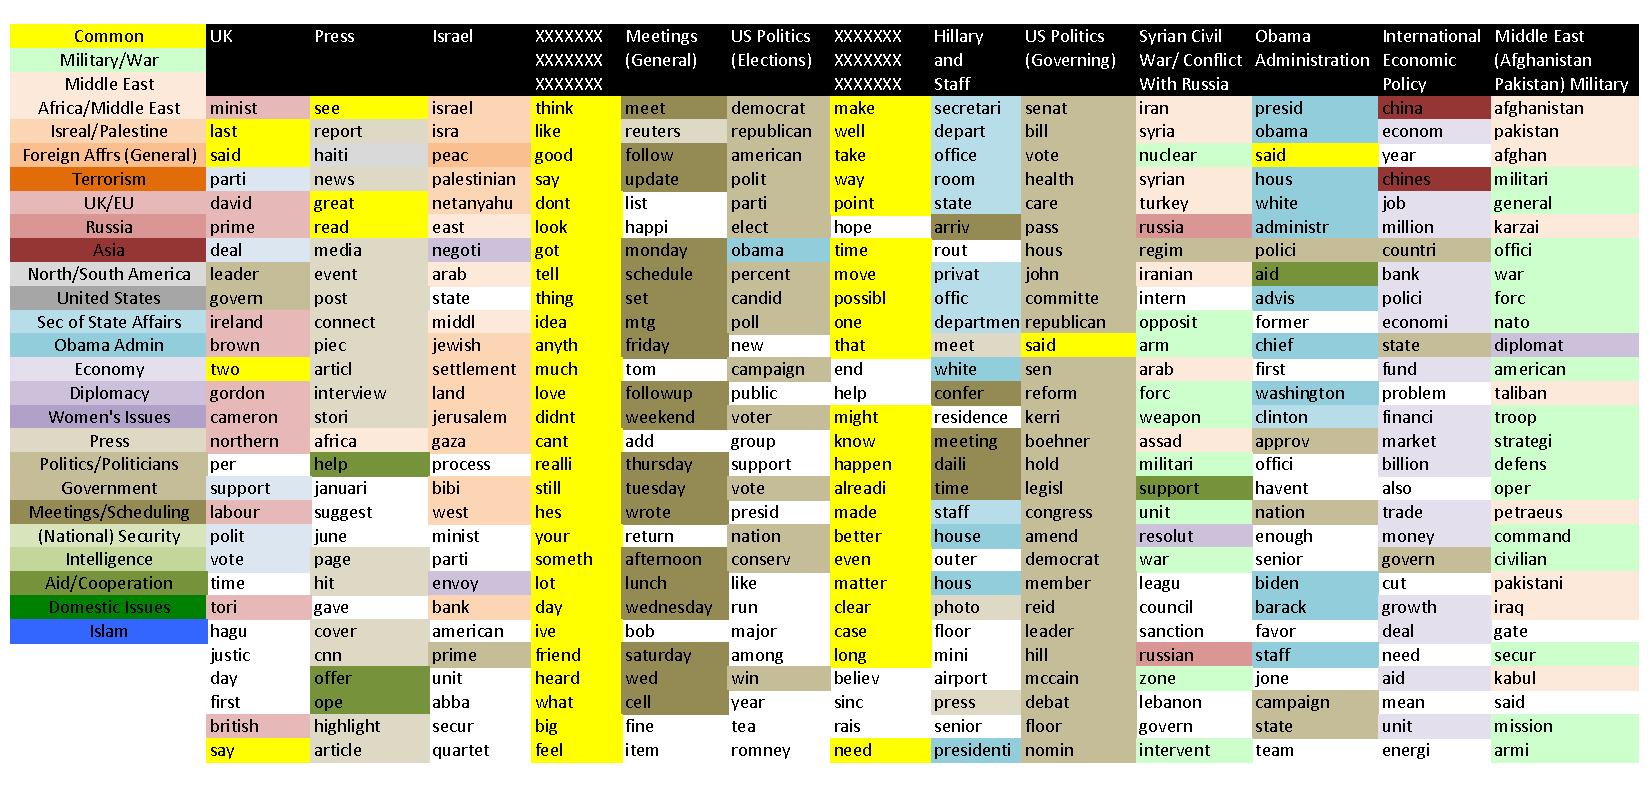
\includegraphics[width=0.99\linewidth]{../images/topic_words.pdf}
\label{fig:topics}
\end{figure}
\end{frame}


\begin{frame}{Primary Topic Frequency}
\begin{columns}

  \column{.7\textwidth}
  \begin{figure}[h]
  \centering
  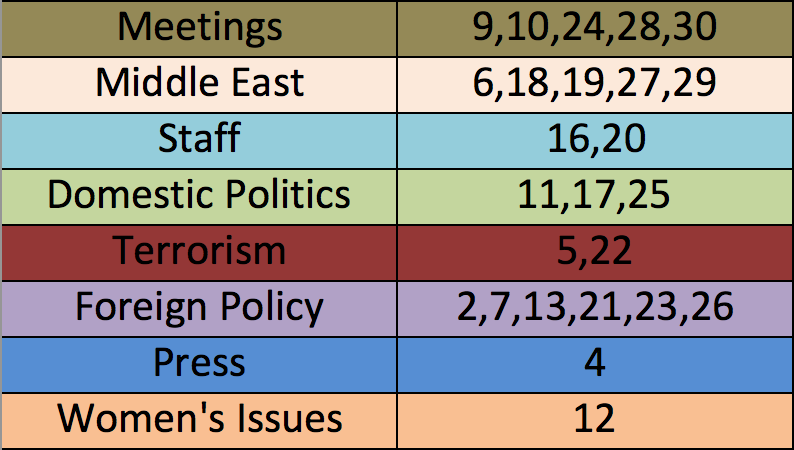
\includegraphics[width=0.8\linewidth]{../images/topic_desc.png}
  \label{fig:topics_desc}
  \end{figure}

  \column{.3\textwidth}
  \begin{figure}[h]
  \centering
  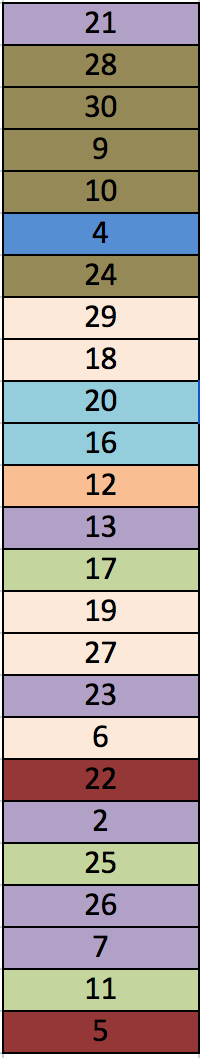
\includegraphics[height=0.75\textheight]{../images/topic_freq.png}
  \label{fig:topics_freq}
  \end{figure}

\end{columns}
\end{frame}


\begin{frame}{Some ``Not'' Interesting Topics}
\begin{table}[h]
\centering
\label{topic_common_words}
\scalebox{0.8}{
\begin{tabular}{cccccc}
\toprule
Common 1 & Common 2 & Common 3 & Logistics & Meeting & Communication \\
\midrule
know & think & will & secretari & meet & call \\
just & like & work & depart & reuters & huma \\
want & good & week & office & follow & abedin \\
let & say & need & room & update & schedul \\
ask & dont & next & state & list & sheet \\
come & look & also & arriv & happi & request \\
tri & got & plan & rout & monday & speak \\
sure & tell & start & privat & schedule & readout \\
thx & thing & issu & office & set & calls \\
\bottomrule
\end{tabular}
}
\end{table}
\end{frame}


\begin{frame}{Some Interesting Topics}
\begin{table}[h]
\centering
\label{topic_top_words}
\scalebox{0.8}{
\begin{tabular}{cccccc}
\toprule
Israel & Elections & Libya & Afghanistan & Int. Dev. & Obama \\
\midrule
israel & democrat & libya & afghanistan & develop & presid \\
isra & republican & secur & pakistan & state & obama \\
peace & american & travel & afghan & support & said \\
palestinian & polit & libyan & militari & global & hous \\
netanyahu & parti & iraq & general & program & white \\
east & elect & embassi & karzai & effort & administr \\
negoti & obama & attack & offici & intern & polici \\
arab & percent & kill & war & work & aid \\
state & candid & march & forc & includ & advis \\
\bottomrule
\end{tabular}
}
\end{table}
\end{frame}


\begin{frame}{Topic Importance Over Time}
\begin{figure}[h]
\centering
\subfigure[Israel]{\label{fig:t1}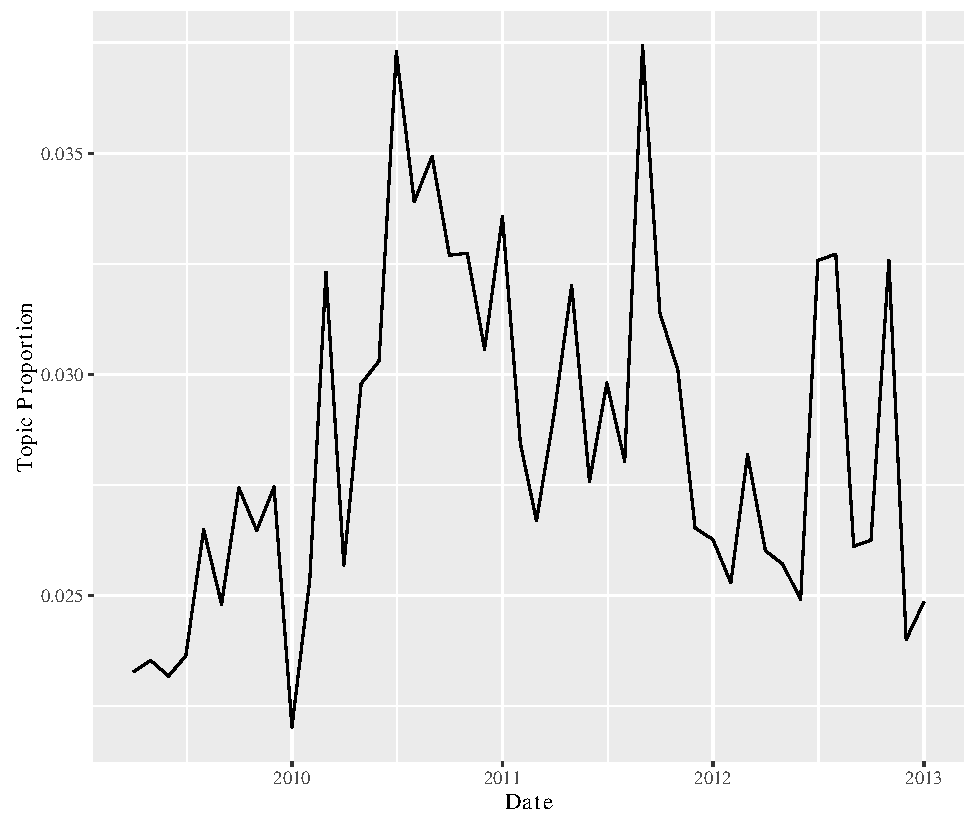
\includegraphics[width=0.25\linewidth]{../images/time_plot6.pdf}}
\subfigure[Elections]{\label{fig:t2}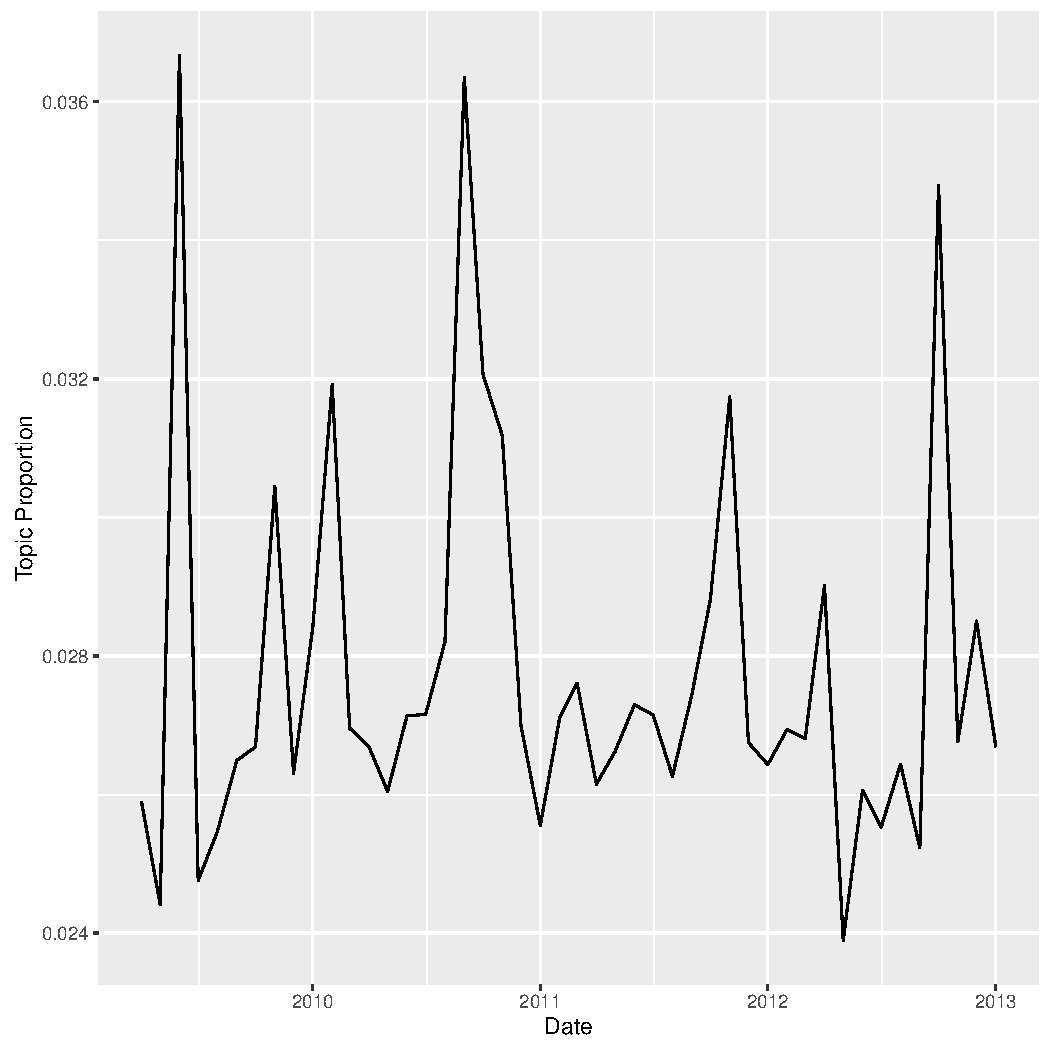
\includegraphics[width=0.25\linewidth]{../images/time_plot11.pdf}}
\subfigure[Libya]{\label{fig:t3}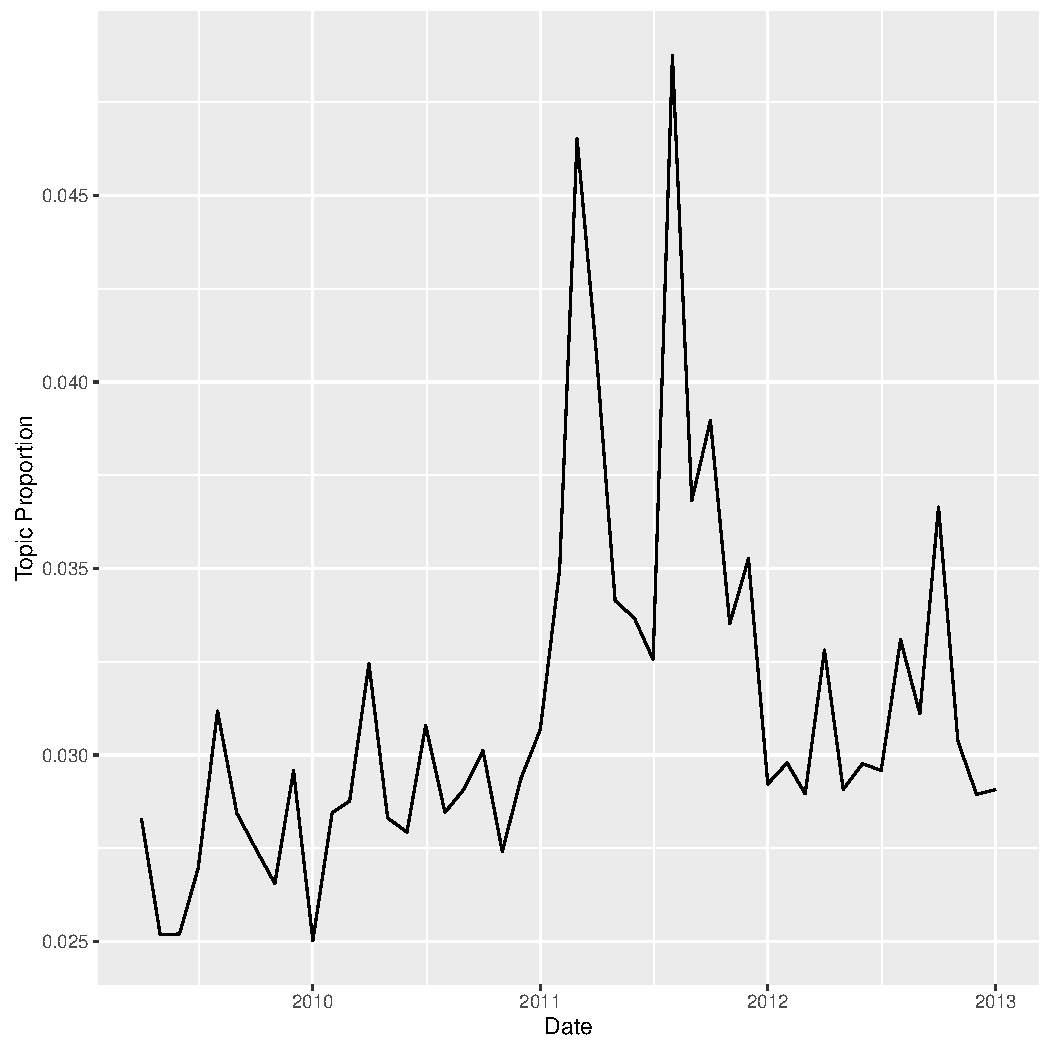
\includegraphics[width=0.25\linewidth]{../images/time_plot18.pdf}}
\subfigure[Afghanistan]{\label{fig:t4}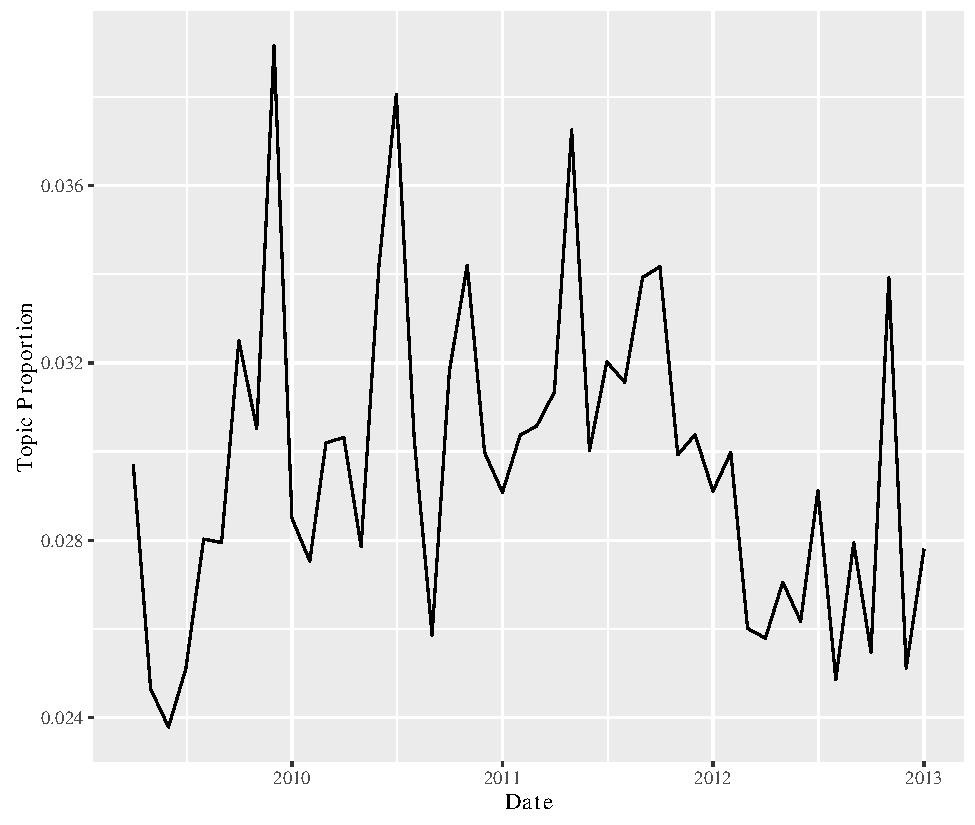
\includegraphics[width=0.25\linewidth]{../images/time_plot27.pdf}}
\subfigure[Int. Dev.]{\label{fig:t5}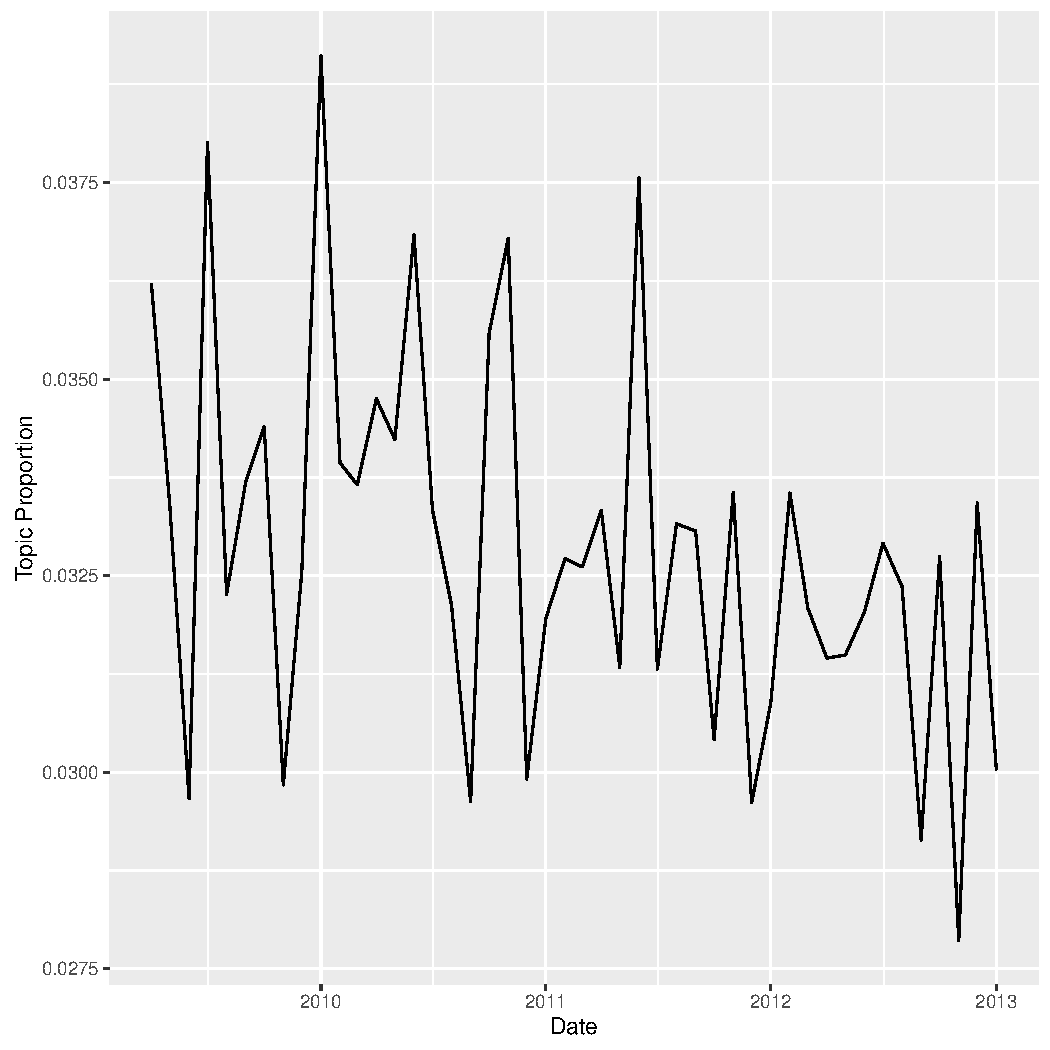
\includegraphics[width=0.25\linewidth]{../images/time_plot23.pdf}}
\subfigure[Obama]{\label{fig:t6}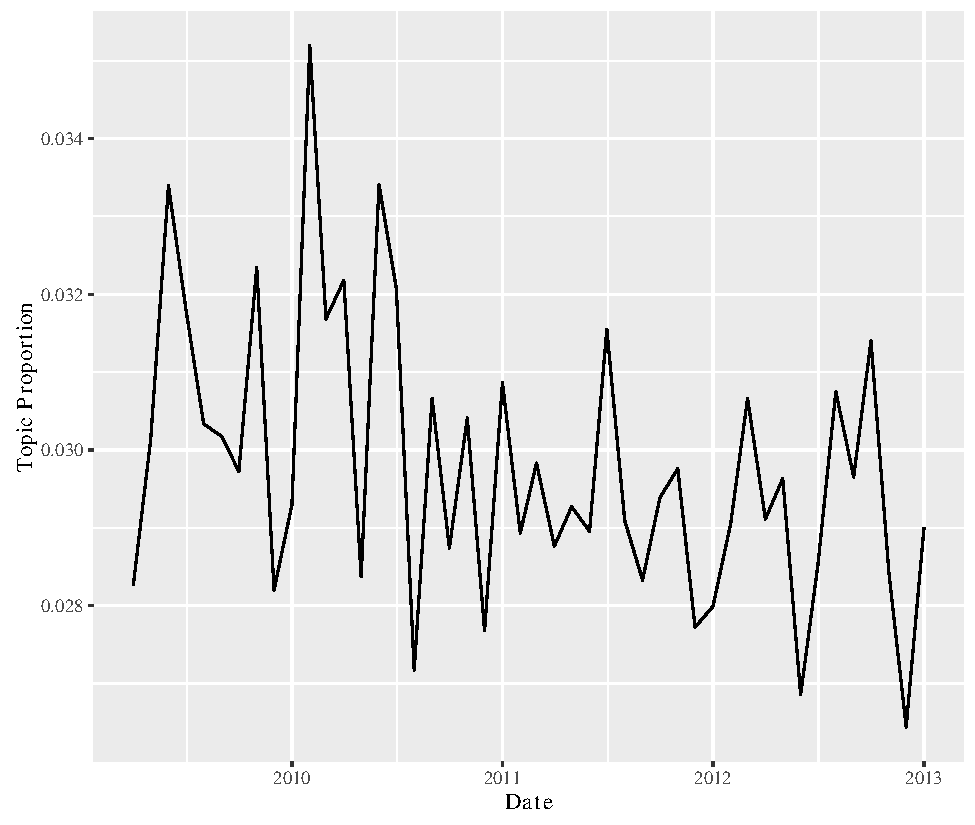
\includegraphics[width=0.25\linewidth]{../images/time_plot25.pdf}}
\label{fig:topic_time_plots}
\end{figure}
\end{frame}


\begin{frame}{Who Says What?}
\begin{table}[h]
\centering
\label{topic_sources}
\scalebox{0.58}{
\begin{tabular}{cccccc}
\toprule
Israel & Elections & Libya & Afghanistan & Int. Dev. & Obama \\
\midrule
Sidney Blumenthal & SB & Huma Abedin & Judith McHale & JM & SB \\
(SB) & & (HA) & (JM) & & \\
\noalign{\vskip 7mm}
HA & Philippe Reines & Wendy Sherman & HA & Melanne Verveer & PR \\
& (PR) & (WS) & & (MV) & \\
\noalign{\vskip 7mm}
Jake Sullivan & JM & JS & MV & Anne-Marie & Cherly Mills \\
(JS) & & & & Slaughter (AMS) & (CM)\\
\noalign{\vskip 7mm}
AMS & CM & Monica Hanley & JS & CM & HA \\
& & (MH) & & & \\
\noalign{\vskip 7mm}
Hillary Clinton & HA & SB & Richard Verma & JS & HC \\
(HC) & & & (RV) & & \\
\bottomrule
\end{tabular}
}
\end{table}
\end{frame}


\begin{frame}{Multinomial Logistic Regression}
\begin{itemize}
\item Can we do a better job associating email senders with topics?
\item To answer this question we employ multinomial regression.
\item We take a subset of people who sent emails, only those who have more that 100 emails sent and try to predict the sender using the topics.
\end{itemize}
\end{frame}


\begin{frame}{Multinomial Logistic Regression Results}
\begin{table}[h]
\centering
\label{multinomial_results}
\scalebox{0.7}{
\begin{tabular}{ccc}
\toprule
Source & Success Rate & Testing Observations \\
\midrule
Hillary Clinton & 0.74 & 849 \\
Philippe Reines & 0.06 & 34 \\
Claire Coleman & 0.52 & 27 \\
Lauren Jiloty & 0.42 & 71 \\
Huma Abedin & 0.36 & 376 \\
Jake Sullivan & 0.23 & 410 \\
Sidney Blumenthal & 0.29 & 87 \\
Cherly Mills & 0.31 & 491 \\
Anne-Marie Slaughter & 0.36 & 42 \\
Monica Hanley & 0.09 & 53 \\
Judith McHale & 0.25 & 28 \\
Robert Russo & 0.00 & 10 \\
Richard Verma & 0.26 & 19 \\
Wendy Sherman & 0.08 & 12 \\
Melanne Verveer & 0.30 & 30 \\
Lona Valmoro & 0.34 & 41 \\
\bottomrule
\end{tabular}
}
\end{table}
\end{frame}


\begin{frame}{Conclusion}
\begin{itemize}
\item We've broken the corpus down to a level where we can effectively analyze it and draw conclusions using both human and statistical analysis
\item This has only been a sample of the many questions we could address using the LDA output
\item Possible future directions
  \begin{itemize}
  \item Some emails are redacted, how do email topics relate to this
  \item Correlation between topics, what topics appear together
  \item Incorporating information on receivers 
  \end{itemize}
\item If this data intrigues you, all the code we used to download, process, and analyze the data is (will be) available at \url{https://github.com/lbybee/601_Final_Project}.
\end{itemize}
\end{frame}



\end{document}
